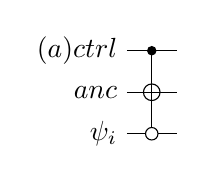
\begin{tikzpicture}[scale=1.000000,x=1pt,y=1pt]
\filldraw[color=white] (0.000000, -7.500000) rectangle (18.000000, 37.500000);
% Drawing wires
% Line 1: ctrl W \text{(a) }ctrl
\draw[color=black] (0.000000,30.000000) -- (18.000000,30.000000);
\draw[color=black] (0.000000,30.000000) node[left] {$\text{(a) }ctrl$};
% Line 2: anc W anc
\draw[color=black] (0.000000,15.000000) -- (18.000000,15.000000);
\draw[color=black] (0.000000,15.000000) node[left] {$anc$};
% Line 3: i W \psi_i
\draw[color=black] (0.000000,0.000000) -- (18.000000,0.000000);
\draw[color=black] (0.000000,0.000000) node[left] {$\psi_i$};
% Done with wires; drawing gates
% Line 5: -i +anc ctrl
\draw (9.000000,30.000000) -- (9.000000,0.000000);
\draw[fill=white] (9.000000, 0.000000) circle(2.250000pt);
\begin{scope}
\draw[fill=white] (9.000000, 15.000000) circle(3.000000pt);
\clip (9.000000, 15.000000) circle(3.000000pt);
\draw (6.000000, 15.000000) -- (12.000000, 15.000000);
\draw (9.000000, 12.000000) -- (9.000000, 18.000000);
\end{scope}
\filldraw (9.000000, 30.000000) circle(1.500000pt);
% Done with gates; drawing ending labels
% Done with ending labels; drawing cut lines and comments
% Done with comments
\end{tikzpicture}
